% Five elements of the dihedral group D_10 (= symmetries of a regular
% pentagon), each shown as a labeled pentagon: 1 (identity), r (rotate
% by 2π/5), s (reflect across the line through vertex 1), sr, rs.
% Source: book/tex/H113/grp-intro.tex (§ Definition and examples).
\documentclass[border=2mm]{standalone}
\usepackage{tikz}
\begin{document}
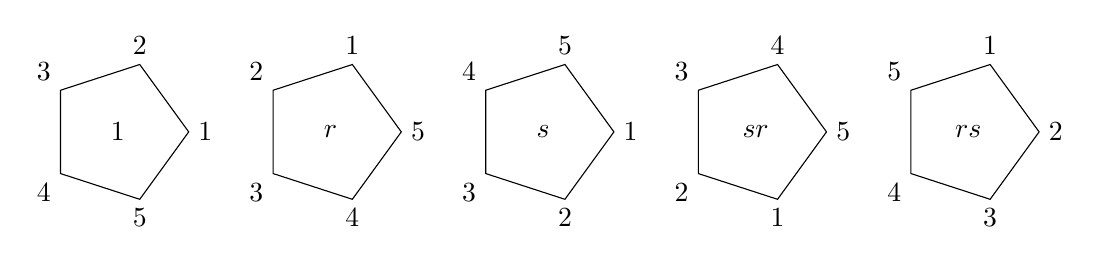
\begin{tikzpicture}[scale=0.9]
  % --- Helper: \pentagon{xshift}{label}{v0}{v1}{v2}{v3}{v4} ---
  % Draws a regular pentagon centred at (xshift, 0) with vertices labelled
  % v0..v4 at angles 0°, 72°, 144°, 216°, 288°, and {label} at the centre.
  \newcommand{\pentagon}[7]{%
    \begin{scope}[shift={(#1,0)}]
      \draw ({cos(0)}, {sin(0)})
        -- ({cos(72)},  {sin(72)})
        -- ({cos(144)}, {sin(144)})
        -- ({cos(216)}, {sin(216)})
        -- ({cos(288)}, {sin(288)})
        -- cycle;
      \node at ({cos(0)},   {sin(0)})   [right]      {$#3$};
      \node at ({cos(72)},  {sin(72)})  [above]      {$#4$};
      \node at ({cos(144)}, {sin(144)}) [above left] {$#5$};
      \node at ({cos(216)}, {sin(216)}) [below left] {$#6$};
      \node at ({cos(288)}, {sin(288)}) [below]      {$#7$};
      \node at (0,0) {$#2$};
    \end{scope}}
  % Identity, then rotation, reflection, and two compositions.
  \pentagon{0}{1}{1}{2}{3}{4}{5}
  \pentagon{3}{r}{5}{1}{2}{3}{4}
  \pentagon{6}{s}{1}{5}{4}{3}{2}
  \pentagon{9}{sr}{5}{4}{3}{2}{1}
  \pentagon{12}{rs}{2}{1}{5}{4}{3}
\end{tikzpicture}
\end{document}
